\documentclass{article}

\usepackage[latin1]{inputenc}
\usepackage{tikz}
\usetikzlibrary{decorations.markings}

\tikzset
 {every pin/.style = {pin edge = {<-}},    % pins are arrows from label to point
  > = stealth,                            % arrow tips look like stealth bombers
  flow/.style =    % everything marked as "flow" will be decorated with an arrow
   {decoration = {markings, mark=at position #1 with {\arrow{>}}},
    postaction = {decorate}
   },
  flow/.default = 0.5,          % default position of the arrow is in the middle
  main/.style = {line width=1pt}                    % thick lines for main graph
 }

% GNUPLOT required
\begin{document}
\pagestyle{empty}


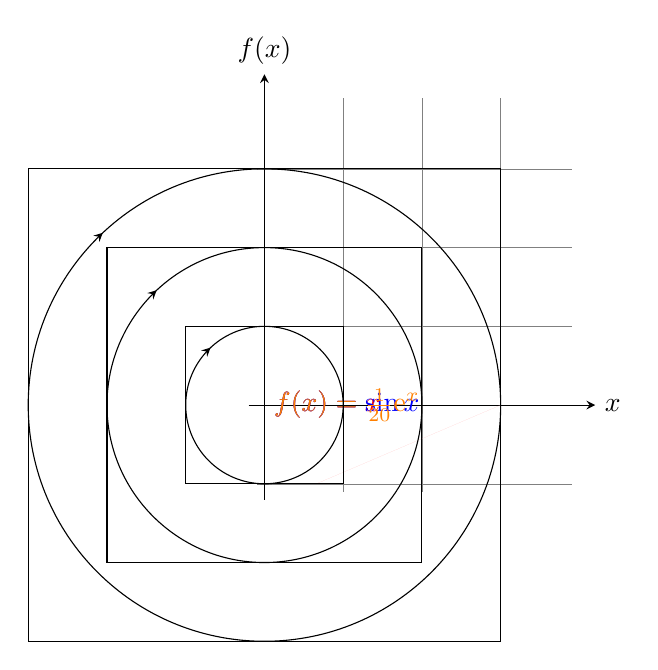
\begin{tikzpicture}[domain=0:4]
    \draw[very thin,color=gray] (-0.1,-1.1) grid (3.9,3.9);
    \draw[->] (-0.2,0) -- (4.2,0) node[right] {$x$};
    \draw[->] (0,-1.2) -- (0,4.2) node[above] {$f(x)$};
    \draw[color=red] plot[id=x] function{x} 
        node[right] {$f(x) =x$};
    \draw[color=blue] plot[id=sin] function{sin(x)} 
        node[right] {$f(x) = \sin x$};
    \draw[color=orange] plot[id=exp] function{0.05*exp(x)} 
        node[right] {$f(x) = \frac{1}{20} \mathrm e^x$};
    \fill[red!30] (0.658,-1)  -- plot[id=f3,domain=0.658:3,samples=50]
        function {0.05*exp(x)} -- (3,0) -- cycle;
    \foreach \r in {1,2,3}                  % draw three circles
    {
        \draw[flow=0.63] (\r,0) arc (0:-360:\r cm);
        \draw (\r,\r) rectangle (-\r, -\r);
    }

\end{tikzpicture}


\begin{tikzpicture}[even odd rule,rounded corners=2pt,x=10pt,y=10pt]
    \filldraw[fill=yellow!80!black] (0,0) rectangle (1,1)
        [xshift=5pt,yshift=5pt] (0,0) rectangle (1,1)
        [rotate=30] (-1,-1) rectangle (2,2);
\end{tikzpicture}

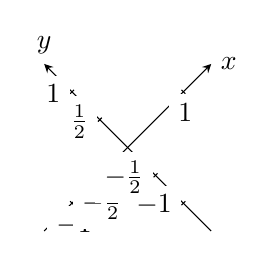
\begin{tikzpicture}
    \begin{scope}[rotate=45]
        \draw[->] (-1.5,0) -- (1.5,0) node[right] {$x$} coordinate(x axis);
        \draw[->] (0,-1.5) -- (0,1.5) node[above] {$y$} coordinate(y axis);
        \foreach \x/\xtext in {-1, -.5/-\frac{1}{2}, 1}
        \draw[xshift=\x cm] (0pt,1pt) -- (0pt,-1pt) node[below,fill=white] {$\xtext$};
        \foreach \y/\ytext in {-1, -.5/-\frac{1}{2}, .5/\frac{1}{2}, 1}
        \draw[yshift=\y cm] (1pt,0pt) -- (-1pt,0pt) node[left,fill=white] {$\ytext$};
    \end{scope}
\end{tikzpicture}

\end{document}
